\chapter{Формализация процесса создания эмуляторов аппаратного обеспечения}\label{ch:ch2}

Помимо сказанного в главе \ref{sec:ch1/sec4} для создании эмуляторов аппаратного обеспечения
требуется формализовать данную задачу.

\section{Подход}\label{sec:ch2/sec1}

Подход к решению обозначенных проблем будет основываться на эмуляторе QEMU и его
возможности встраивать пользовательские устройства.
Для этого необходимо:

\begin{enumerate}[label={\arabic*)}]
    \item \label{q-inh} проанализировать цепочки наследования сущностей QOM;
    \item \label{q-inh-scheme} составить схему наследования сущностей;
    \item \label{q-interface} определить интерфейс взаимодействия эмулятора с выделенными сущностями;
    \item \label{q-impl} реализовать устройство;
\end{enumerate}

Корректность выполнения пунктов \ref{q-inh}-\ref{q-interface} должна полностью брать на себя разрабатываемая система,
тогда как вместо предоставления автосгенерированного файла с исходным кодом \ref{sec:ch1/sec2} для
последующей модификации, результатом выполнения пункта \ref{q-impl} должен быть готовый к встраиванию
файл с исходным кодом, не требующий ручной модификации.
Для этого требуется проблемно-ориентированный язык, компиляция которого, помимо генерации шаблонного кода
создаст интерфейс передачи объектов между C-устройством внутри QEMU и интерпретатором Python, в
котором будет исполняться реализованная логика работы устройства.

С учетом всего вышесказанного, На рис. \ref{fig:device-compilation} показана функциональная схема преобразования
описания виртуального устройства в часть эмулятора QEMU.

\begin{figure}[!htbp]
    \centering
    % !TEX encoding = UTF-8 Unicode
% Úτƒ-8 encoded
% http://www.linux.org.ru/forum/general/10357036
\tikzset{
    line/.style={draw, -latex'},
    every join/.style={line},
    u/.style={anchor=south},
    r/.style={anchor=west},
    fxd/.style={text width = 6em},
    it/.style={font={\small\itshape}},
    bf/.style={font={\small\bfseries}},
}
\tikzstyle{base_long} =
    [
        draw,
        on chain,
        on grid,
        align=center,
        minimum height=4ex,
        minimum width = 10ex,
        node distance = 6mm and 60mm,
        text badly centered,
    ]
\tikzstyle{base} =
    [
        draw,
        on chain,
        on grid,
        align=center,
        minimum height=4ex,
        minimum width = 10ex,
        node distance = 6mm and 60mm,
        text badly centered,
        text width=5cm
    ]
\tikzstyle{coord} =
    [
        coordinate,
        on chain,
        on grid
    ]
\tikzstyle{cloud} =
    [
        base,
        ellipse,
        node distance = 3cm,
        minimum height = 2em,
        text width=2cm
    ]
\tikzstyle{decision} =
    [
        base,
        diamond,
        aspect=2,
        node distance = 2cm,
        inner sep = 0pt
    ]
\tikzstyle{block} =
    [
        rectangle,
        base,
        rounded corners,
        minimum height = 2em
    ]
\tikzstyle{print_block} =
    [
        base,
        tape,
        tape bend top=none,
    ]
\tikzstyle{io} =
    [
        base,
        trapezium,
        trapezium left angle = 70,
        trapezium right angle = 110,
    ]
\tikzstyle{prompt} =
    [
        base,
        trapezium,
        trapezium left angle = 90,
        trapezium right angle = 80,
        shape border rotate = 90
    ]
\tikzstyle{disk file} =
    [
        base,
        cylinder,
        aspect=0.2,
    ]
\tikzstyle{process} =
    [
        rectangle,
        base,
    ]
\makeatletter
\pgfkeys{/pgf/.cd,
    subrtshape w/.initial=2mm,
    cycleshape w/.initial=2mm
}
\pgfdeclareshape{parallelshape}{
    \inheritsavedanchors[from=rectangle]
    \inheritanchorborder[from=rectangle]
    \inheritanchor[from=rectangle]{north}
    \inheritanchor[from=rectangle]{center}
    \inheritanchor[from=rectangle]{west}
    \inheritanchor[from=rectangle]{east}
    \inheritanchor[from=rectangle]{mid}
    \inheritanchor[from=rectangle]{base}
    \inheritanchor[from=rectangle]{south}
    \backgroundpath{
        \southwest \pgf@xa=\pgf@x \pgf@ya=\pgf@y
        \northeast \pgf@xb=\pgf@x \pgf@yb=\pgf@y
        \def\ppd@offset{\pgfpoint{\pgfutil@tempdima}{0ex}}
        \def\ppd@offsetm{\pgfpoint{-\pgfutil@tempdima}{0ex}}
        \pgfpathmoveto{\pgfqpoint{\pgf@xa}{\pgf@ya}}
            \pgfpathlineto{\pgfqpoint{\pgf@xb}{\pgf@ya}}
        \pgfpathclose
        \pgfpathmoveto{\pgfqpoint{\pgf@xb}{\pgf@yb}}
            \pgfpathlineto{\pgfqpoint{\pgf@xa}{\pgf@yb}}
        \pgfpathclose
    }
}
\pgfdeclareshape{subrtshape}{
    \inheritsavedanchors[from=rectangle]
    \inheritanchorborder[from=rectangle]
    \inheritanchor[from=rectangle]{north}
    \inheritanchor[from=rectangle]{center}
    \inheritanchor[from=rectangle]{west}
    \inheritanchor[from=rectangle]{east}
    \inheritanchor[from=rectangle]{mid}
    \inheritanchor[from=rectangle]{base}
    \inheritanchor[from=rectangle]{south}
    \backgroundpath{
        \southwest \pgf@xa=\pgf@x \pgf@ya=\pgf@y
        \northeast \pgf@xb=\pgf@x \pgf@yb=\pgf@y
        \pgfmathsetlength\pgfutil@tempdima{\pgfkeysvalueof{/pgf/subrtshape w}}
        \def\ppd@offset{\pgfpoint{\pgfutil@tempdima}{0ex}}
        \def\ppd@offsetm{\pgfpoint{-\pgfutil@tempdima}{0ex}}
        \pgfpathmoveto{\pgfqpoint{\pgf@xa}{\pgf@ya}}
        \pgfpathlineto{\pgfqpoint{\pgf@xb}{\pgf@ya}}
        \pgfpathlineto{\pgfqpoint{\pgf@xb}{\pgf@yb}}
        \pgfpathlineto{\pgfqpoint{\pgf@xa}{\pgf@yb}}
        \pgfpathclose
        \pgfpathmoveto{\pgfpointadd{\pgfpoint{\pgf@xa}{\pgf@yb}}{\ppd@offsetm}}
        \pgfpathlineto{\pgfpointadd{\pgfpoint{\pgf@xa}{\pgf@ya}}{\ppd@offsetm}}
        \pgfpathlineto{\pgfpointadd{\pgfpoint{\pgf@xb}{\pgf@ya}}{\ppd@offset}}
        \pgfpathlineto{\pgfpointadd{\pgfpoint{\pgf@xb}{\pgf@yb}}{\ppd@offset}}
        \pgfpathclose
    }
}
\pgfdeclareshape{cyclebegshape}{
    \inheritsavedanchors[from=rectangle]
    \inheritanchorborder[from=rectangle]
    \inheritanchor[from=rectangle]{north}
    \inheritanchor[from=rectangle]{center}
    \inheritanchor[from=rectangle]{west}
    \inheritanchor[from=rectangle]{east}
    \inheritanchor[from=rectangle]{mid}
    \inheritanchor[from=rectangle]{base}
    \inheritanchor[from=rectangle]{south}
    \backgroundpath{
        \southwest \pgf@xa=\pgf@x \pgf@ya=\pgf@y
        \northeast \pgf@xb=\pgf@x \pgf@yb=\pgf@y
        \pgfmathsetlength\pgfutil@tempdima{\pgfkeysvalueof{/pgf/cycleshape w}}
        \pgfpathmoveto{\pgfqpoint{\pgf@xa}{\pgf@ya}}
\pgfpathlineto{\pgfpointadd{\pgfpoint{\pgf@xa}{\pgf@yb}}{\pgfpoint{0ex}{-\pgfutil@tempdima}}}
\pgfpathlineto{\pgfpointadd{\pgfpoint{\pgf@xa}{\pgf@yb}}{\pgfpoint{\pgfutil@tempdima}{0ex}}}
\pgfpathlineto{\pgfpointadd{\pgfpoint{\pgf@xb}{\pgf@yb}}{\pgfpoint{-\pgfutil@tempdima}{0ex}}}
\pgfpathlineto{\pgfpointadd{\pgfpoint{\pgf@xb}{\pgf@yb}}{\pgfpoint{0ex}{-\pgfutil@tempdima}}}
\pgfpathlineto{\pgfqpoint{\pgf@xb}{\pgf@ya}}
        \pgfpathclose
    }
}
\pgfdeclareshape{cycleendshape}{
    \inheritsavedanchors[from=rectangle]
    \inheritanchorborder[from=rectangle]
    \inheritanchor[from=rectangle]{north}
    \inheritanchor[from=rectangle]{center}
    \inheritanchor[from=rectangle]{west}
    \inheritanchor[from=rectangle]{east}
    \inheritanchor[from=rectangle]{mid}
    \inheritanchor[from=rectangle]{base}
    \inheritanchor[from=rectangle]{south}
    \backgroundpath{
        \southwest \pgf@xa=\pgf@x \pgf@ya=\pgf@y
        \northeast \pgf@xb=\pgf@x \pgf@yb=\pgf@y
        \pgfmathsetlength\pgfutil@tempdima{\pgfkeysvalueof{/pgf/cycleshape w}}
        \pgfpathmoveto{\pgfqpoint{\pgf@xb}{\pgf@yb}}
\pgfpathlineto{\pgfpointadd{\pgfpoint{\pgf@xb}{\pgf@ya}}{\pgfpoint{0ex}{\pgfutil@tempdima}}}
\pgfpathlineto{\pgfpointadd{\pgfpoint{\pgf@xb}{\pgf@ya}}{\pgfpoint{-\pgfutil@tempdima}{0ex}}}
\pgfpathlineto{\pgfpointadd{\pgfpoint{\pgf@xa}{\pgf@ya}}{\pgfpoint{\pgfutil@tempdima}{0ex}}}
\pgfpathlineto{\pgfpointadd{\pgfpoint{\pgf@xa}{\pgf@ya}}{\pgfpoint{0ex}{\pgfutil@tempdima}}}
\pgfpathlineto{\pgfqpoint{\pgf@xa}{\pgf@yb}}
        \pgfpathclose
    }
}
\makeatother
\tikzstyle{subroutine} =
    [
        base,
        subrtshape,
    ]
\tikzstyle{cyclebegin} =
    [
        base,
        cyclebegshape,
    ]
\tikzstyle{cycleend} =
    [
        base,
        cycleendshape,
    ]
\tikzstyle{connector} =
    [
        base,
        circle,
    ]

\tikzstyle{parallel} =
    [
        base_long,
        parallelshape,
    ]
\begin{tikzpicture}[%
    start chain=going below,    % General flow is top-to-bottom
    node distance=6mm and 30mm, % Global setup of box spacing
    ]
        \node  [rectangle,
                base,
                dotted,
                minimum width=6cm,
                minimum height=15cm] (compile rect) at (0,-10) {};

        \node [color = blue, left = 1cm of compile rect, yshift = 0.25cm]  (group) {\small Компиляция устройства};
        \draw [color = blue, decorate, decoration = {brace,amplitude=10pt,raise=5pt, mirror}] (-3cm,-2cm) --  (-3cm,-17cm);


        \node  [cloud] (begin) at (0,0) {\small Начало};
        \node  [subroutine]   (parse)          [below = 2cm of begin]            {\small Разбор файла};
        \node  [subroutine]   (qemu inh)       [below = 2cm of parse]            {\small Поиск используемых\\сущностей QEMU};
        \node  [subroutine]   (qemu inh inter) [below = 2.2cm of qemu inh]       {\small Определение интерфейса используемых\\сущностей QEMU};
        \node  [subroutine]   (qemu inh boil)  [below = 2.2cm of qemu inh inter] {\small Генерация C-интерфейса устройства в QEMU};
        \node  [subroutine]   (python)         [below = 2.2cm of qemu inh boil]  {\small Генерация python-интерфейса\\для логики устройства};
        \node  [subroutine]   (buildsystem)    [below = 2.2cm of python]         {\small Встраивание устройства\\в сборку QEMU};

        \node  [disk file] (source)         [left  = 8cm of parse]            {\small Исходный код устройства};
        \node  [disk file] (qemu folder)    [left  = 8cm of buildsystem]      {\small Сборочная папка QEMU};
        \node  [subroutine] (compile)       [below = 3cm of buildsystem]      {\small Сборка QEMU};
        \node  [disk file] (binary)         [left  = 8cm of compile]        {\small QEMU со встроенным устройством};

        \node  [cloud] (end) [below = 2cm of compile] {\small Конец};

        \draw [->] (begin)          -- (parse);
        \draw [->] (source)         -- (parse);
        \draw [->] (parse)          -- (qemu inh);
        \draw [->] (qemu inh)       -- (qemu inh inter);
        \draw [->] (qemu inh inter) -- (qemu inh boil);
        \draw [->] (qemu inh boil)  -- (python);
        \draw [->] (python)         -- (buildsystem);
        \draw [->] (qemu folder)    -- (buildsystem);
        \draw [->] (buildsystem)    -- (compile);
        \draw [->] (compile)        -- (binary);
        \draw [->] (compile)        -- (end);


\end{tikzpicture}

    \caption{Функциональная схема компиляции виртуального устройства.}\label{fig:device-compilation}
\end{figure}


\subsection{Язык описания виртуального устройства}\label{sec:ch2/sec1/sub1}

Использование специализированного языка для описания устройства, в отличие от языка общего назначения (см. \ref{sec:ch1/sec2}),
имеет как определенные преимущества, так и недостатки.
К преимуществам можно отнести:
\begin{itemize}
    \item ограничение пользователя языка только необходимыми конструкциями -- минимизация ошибок программирования;
    \item точные, по сравнению с языком общего назначения, сообщения об ошибках;
    \item самодокументируемость решения проблемы;
    \item более эффективная, по времени, разработка.
\end{itemize}

К недостаткам -- необходимость предварительного изучения проблемно-ориентированного языка.
Как можно убедиться, преимуществ, несмотря на определенную трудоемкость разработки такого языка,
больше.
Необходимость изучения дополнительного языка для описания виртуального устройства может показаться
избыточной, но использование языка общего назначения (см. \ref{sec:ch1/sec2}),
пусть и популярного, не гарантирует, что пользователь его знает и эффективно в нем работает.
Помимо этого, изучение небольшого языка для решения конкретной проблемы будет эффективнее
изучения библиотеки и некоторого подмножества полноценного языка программирования,
из которого ее можно будет использовать.

Ограничение в языковых конструкциях и анализ семантики исходного кода
позволяет точно инструктировать пользователя об ошибках в реализации виртуального устройства,
что ведет к отсутствию ошибок уровня интерфейса устройства,
сводя появление возможных неисправностей только до реализации логики устройства.

Язык-фреймворк Racket \cite{racket-lang} разработан как раз для языково-ориентированного
программирования. Написание на нем логики компилятора или интерпретатора целевого языка
полуавтоматически создает интегрированную среду разработки с помощью IDE DrRacket, которую
также поддерживает сообщество.
После объявления некоторых функций \cite{racket-drracket-integration}, разработчик программ
на целевом языке сможет пользоваться подсветкой синтаксиса, отладчиком, автоматическим добавлением
отступов и указателями использования переменных (рис. \ref{fig:racket-variable-arrow}), что дополнительно облегчает разработку.

\begin{figure}[!htbp]
    \centering
    \begin{adjustbox}{max totalsize={\textwidth}{\textheight}}
        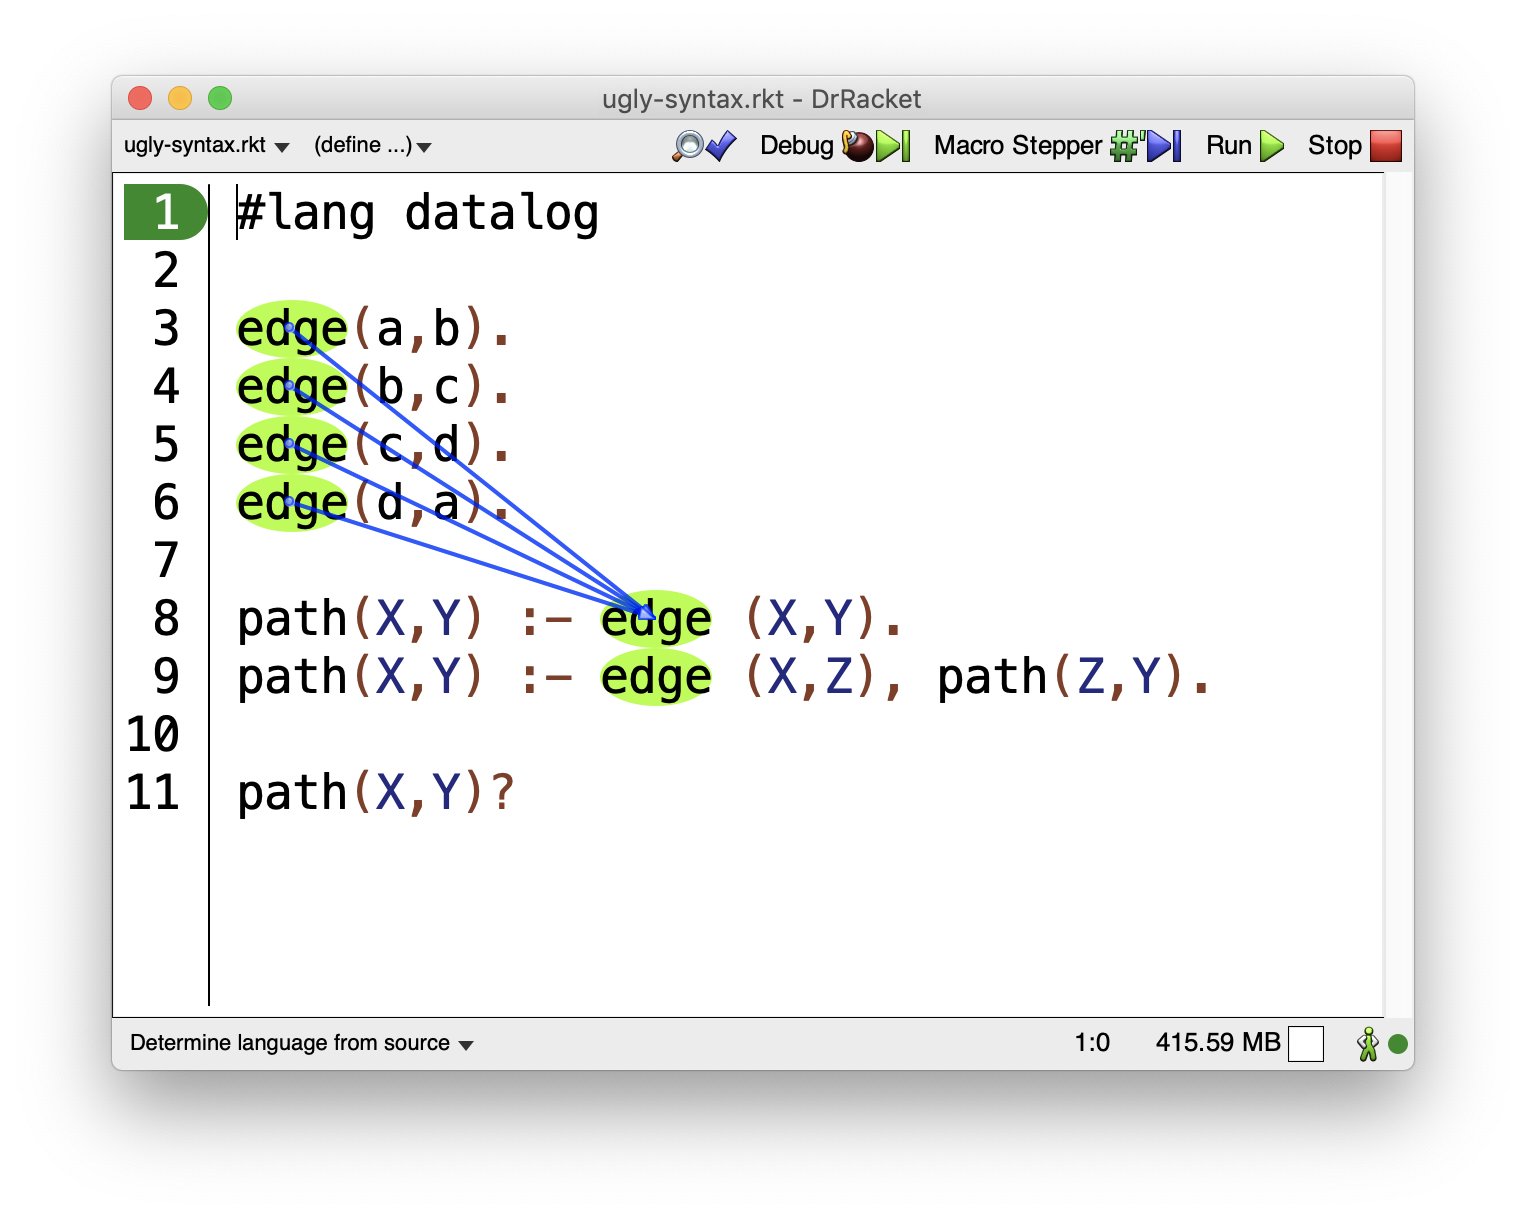
\includegraphics[]{images/racket-variable-arrow.png}
    \end{adjustbox}
    \caption{Результат интеграции языка datalog в IDE DrRacket.}\label{fig:racket-variable-arrow}
\end{figure}


\subsubsection{Структура программы}\label{sec:ch2/sec1/sub1/sub1}

Структура программы-описания аппаратного обеспечения имеет следующий вид, рисунок \ref{fig:device-program-structure}.

\begin{figure}[!htbp]
    \centering
    % !TEX encoding = UTF-8 Unicode
% Úτƒ-8 encoded
% http://www.linux.org.ru/forum/general/10357036
\tikzset{
    line/.style={draw, -latex'},
    every join/.style={line},
    u/.style={anchor=south},
    r/.style={anchor=west},
    fxd/.style={text width = 6em},
    it/.style={font={\small\itshape}},
    bf/.style={font={\small\bfseries}},
}
\tikzstyle{base_long} =
    [
        draw,
        on chain,
        on grid,
        align=center,
        minimum height=4ex,
        minimum width = 10ex,
        node distance = 6mm and 60mm,
        text badly centered,
    ]
\tikzstyle{base} =
    [
        draw,
        on chain,
        on grid,
        align=center,
        minimum height=4ex,
        minimum width = 10ex,
        node distance = 6mm and 60mm,
        text badly centered,
        text width=5cm
    ]
\tikzstyle{coord} =
    [
        coordinate,
        on chain,
        on grid
    ]
\tikzstyle{cloud} =
    [
        base,
        ellipse,
        node distance = 3cm,
        minimum height = 2em,
        text width=2cm
    ]
\tikzstyle{decision} =
    [
        base,
        diamond,
        aspect=2,
        node distance = 2cm,
        inner sep = 0pt
    ]
\tikzstyle{block} =
    [
        rectangle,
        base,
        rounded corners,
        minimum height = 2em
    ]
\tikzstyle{print_block} =
    [
        base,
        tape,
        tape bend top=none,
    ]
\tikzstyle{io} =
    [
        base,
        trapezium,
        trapezium left angle = 70,
        trapezium right angle = 110,
    ]
\tikzstyle{prompt} =
    [
        base,
        trapezium,
        trapezium left angle = 90,
        trapezium right angle = 80,
        shape border rotate = 90
    ]
\tikzstyle{disk file} =
    [
        base,
        cylinder,
        aspect=0.2,
    ]
\tikzstyle{process} =
    [
        rectangle,
        base,
    ]
\makeatletter
\pgfkeys{/pgf/.cd,
    subrtshape w/.initial=2mm,
    cycleshape w/.initial=2mm
}
\pgfdeclareshape{parallelshape}{
    \inheritsavedanchors[from=rectangle]
    \inheritanchorborder[from=rectangle]
    \inheritanchor[from=rectangle]{north}
    \inheritanchor[from=rectangle]{center}
    \inheritanchor[from=rectangle]{west}
    \inheritanchor[from=rectangle]{east}
    \inheritanchor[from=rectangle]{mid}
    \inheritanchor[from=rectangle]{base}
    \inheritanchor[from=rectangle]{south}
    \backgroundpath{
        \southwest \pgf@xa=\pgf@x \pgf@ya=\pgf@y
        \northeast \pgf@xb=\pgf@x \pgf@yb=\pgf@y
        \def\ppd@offset{\pgfpoint{\pgfutil@tempdima}{0ex}}
        \def\ppd@offsetm{\pgfpoint{-\pgfutil@tempdima}{0ex}}
        \pgfpathmoveto{\pgfqpoint{\pgf@xa}{\pgf@ya}}
            \pgfpathlineto{\pgfqpoint{\pgf@xb}{\pgf@ya}}
        \pgfpathclose
        \pgfpathmoveto{\pgfqpoint{\pgf@xb}{\pgf@yb}}
            \pgfpathlineto{\pgfqpoint{\pgf@xa}{\pgf@yb}}
        \pgfpathclose
    }
}
\pgfdeclareshape{subrtshape}{
    \inheritsavedanchors[from=rectangle]
    \inheritanchorborder[from=rectangle]
    \inheritanchor[from=rectangle]{north}
    \inheritanchor[from=rectangle]{center}
    \inheritanchor[from=rectangle]{west}
    \inheritanchor[from=rectangle]{east}
    \inheritanchor[from=rectangle]{mid}
    \inheritanchor[from=rectangle]{base}
    \inheritanchor[from=rectangle]{south}
    \backgroundpath{
        \southwest \pgf@xa=\pgf@x \pgf@ya=\pgf@y
        \northeast \pgf@xb=\pgf@x \pgf@yb=\pgf@y
        \pgfmathsetlength\pgfutil@tempdima{\pgfkeysvalueof{/pgf/subrtshape w}}
        \def\ppd@offset{\pgfpoint{\pgfutil@tempdima}{0ex}}
        \def\ppd@offsetm{\pgfpoint{-\pgfutil@tempdima}{0ex}}
        \pgfpathmoveto{\pgfqpoint{\pgf@xa}{\pgf@ya}}
        \pgfpathlineto{\pgfqpoint{\pgf@xb}{\pgf@ya}}
        \pgfpathlineto{\pgfqpoint{\pgf@xb}{\pgf@yb}}
        \pgfpathlineto{\pgfqpoint{\pgf@xa}{\pgf@yb}}
        \pgfpathclose
        \pgfpathmoveto{\pgfpointadd{\pgfpoint{\pgf@xa}{\pgf@yb}}{\ppd@offsetm}}
        \pgfpathlineto{\pgfpointadd{\pgfpoint{\pgf@xa}{\pgf@ya}}{\ppd@offsetm}}
        \pgfpathlineto{\pgfpointadd{\pgfpoint{\pgf@xb}{\pgf@ya}}{\ppd@offset}}
        \pgfpathlineto{\pgfpointadd{\pgfpoint{\pgf@xb}{\pgf@yb}}{\ppd@offset}}
        \pgfpathclose
    }
}
\pgfdeclareshape{cyclebegshape}{
    \inheritsavedanchors[from=rectangle]
    \inheritanchorborder[from=rectangle]
    \inheritanchor[from=rectangle]{north}
    \inheritanchor[from=rectangle]{center}
    \inheritanchor[from=rectangle]{west}
    \inheritanchor[from=rectangle]{east}
    \inheritanchor[from=rectangle]{mid}
    \inheritanchor[from=rectangle]{base}
    \inheritanchor[from=rectangle]{south}
    \backgroundpath{
        \southwest \pgf@xa=\pgf@x \pgf@ya=\pgf@y
        \northeast \pgf@xb=\pgf@x \pgf@yb=\pgf@y
        \pgfmathsetlength\pgfutil@tempdima{\pgfkeysvalueof{/pgf/cycleshape w}}
        \pgfpathmoveto{\pgfqpoint{\pgf@xa}{\pgf@ya}}
\pgfpathlineto{\pgfpointadd{\pgfpoint{\pgf@xa}{\pgf@yb}}{\pgfpoint{0ex}{-\pgfutil@tempdima}}}
\pgfpathlineto{\pgfpointadd{\pgfpoint{\pgf@xa}{\pgf@yb}}{\pgfpoint{\pgfutil@tempdima}{0ex}}}
\pgfpathlineto{\pgfpointadd{\pgfpoint{\pgf@xb}{\pgf@yb}}{\pgfpoint{-\pgfutil@tempdima}{0ex}}}
\pgfpathlineto{\pgfpointadd{\pgfpoint{\pgf@xb}{\pgf@yb}}{\pgfpoint{0ex}{-\pgfutil@tempdima}}}
\pgfpathlineto{\pgfqpoint{\pgf@xb}{\pgf@ya}}
        \pgfpathclose
    }
}
\pgfdeclareshape{cycleendshape}{
    \inheritsavedanchors[from=rectangle]
    \inheritanchorborder[from=rectangle]
    \inheritanchor[from=rectangle]{north}
    \inheritanchor[from=rectangle]{center}
    \inheritanchor[from=rectangle]{west}
    \inheritanchor[from=rectangle]{east}
    \inheritanchor[from=rectangle]{mid}
    \inheritanchor[from=rectangle]{base}
    \inheritanchor[from=rectangle]{south}
    \backgroundpath{
        \southwest \pgf@xa=\pgf@x \pgf@ya=\pgf@y
        \northeast \pgf@xb=\pgf@x \pgf@yb=\pgf@y
        \pgfmathsetlength\pgfutil@tempdima{\pgfkeysvalueof{/pgf/cycleshape w}}
        \pgfpathmoveto{\pgfqpoint{\pgf@xb}{\pgf@yb}}
\pgfpathlineto{\pgfpointadd{\pgfpoint{\pgf@xb}{\pgf@ya}}{\pgfpoint{0ex}{\pgfutil@tempdima}}}
\pgfpathlineto{\pgfpointadd{\pgfpoint{\pgf@xb}{\pgf@ya}}{\pgfpoint{-\pgfutil@tempdima}{0ex}}}
\pgfpathlineto{\pgfpointadd{\pgfpoint{\pgf@xa}{\pgf@ya}}{\pgfpoint{\pgfutil@tempdima}{0ex}}}
\pgfpathlineto{\pgfpointadd{\pgfpoint{\pgf@xa}{\pgf@ya}}{\pgfpoint{0ex}{\pgfutil@tempdima}}}
\pgfpathlineto{\pgfqpoint{\pgf@xa}{\pgf@yb}}
        \pgfpathclose
    }
}
\makeatother
\tikzstyle{subroutine} =
    [
        base,
        subrtshape,
    ]
\tikzstyle{cyclebegin} =
    [
        base,
        cyclebegshape,
    ]
\tikzstyle{cycleend} =
    [
        base,
        cycleendshape,
    ]
\tikzstyle{connector} =
    [
        base,
        circle,
    ]

\tikzstyle{parallel} =
    [
        base_long,
        parallelshape,
    ]
\begin{tikzpicture}[%
    start chain=going below,    % General flow is top-to-bottom
    node distance=6mm and 30mm, % Global setup of box spacing
    ]
        \node  [rectangle,
                base,
                minimum width=6cm] (device class)
                {Описание класса устройства};
        \node  [rectangle,
                base,
                minimum width=6cm] (c-python api)
                [below = 1.5cm of device class]
                {Связывание функций C-Python интерфейса};
        \node  [rectangle,
                base,
                minimum width=6cm] (py logic)
                [below = 1.85cm of c-python api]
                {Реализация логики работы устройства на Python};



\end{tikzpicture}

    \caption{Структура программы-описания аппаратного обеспечения.}\label{fig:device-program-structure}
\end{figure}

Несмотря на то, что компилятор язык программы-описания располагает
блоки кода в результирующем тексте модуле QEMU в соответствии
с правилами языка C и порядок объявления блоков в исходном файле ему не важен,
данная структура является наиболее понятной и органичной для стороннего разработчика.
Поэтому компилятор принуждает программиста придерживаться её, подобно тому, как
язык Python обязывает использовать отступы для создания блоков кода.


\subsubsection{Граммматика языка}\label{sec:ch2/sec1/sub1/sub2}
Разрабатываемый язык является языком с контекстно-свободной грамматикой.
Далее он будет именоваться как {\mylanguage} (произносится \mylanguageprononciation)

Грамматика {\mylanguage} ограничена до описания зависимостей устройства и QEMU,
связывания функций C и Python, встраивания Python-кода с логикой работы устройства
в файл.


\begin{figure}[!htbp]
    \begin{grammar}
        <letter> ::= `A' | `B' | `C' | `D' | `E' | `F' | `G'
                   | `H' | `I' | `J' | `K' | `L' | `M' | `N'
                   | `O' | `P' | `Q' | `R' | `S' | `T' | `U'
                   | `V' | `W' | `X' | `Y' | `Z' | `a' | `b'
                   | `c' | `d' | `e' | `f' | `g' | `h' | `i'
                   | `j' | `k' | `l' | `m' | `n' | `o' | `p'
                   | `q' | `r' | `s' | `t' | `u' | `v' | `w'
                   | `x' | `y' | `z' ;

        <digit> ::= `0' | `1' | `2' | `3' | `4' | `5' | `6' | `7' | `8' | `9' ;

        <identifier> ::= <letter> , \{ <letter> | <digit> | `\_' \} ;

        <block start> ::= `{';

        <block end> ::= `}';

        <field> ::= <identifier> `=' <identifier> | <block> ;

        <block> ::= <block start> <field> <block end>;

        <device definition> ::= '\#' <identifier>;

        <device class inheritance> ::= `(' <identifier> `:' <identifier> `,' \{ <identifier> \} `)';

        <device class block> ::= <device class inheritance> <block>;

        <bind block> ::= `@bind' <block>;

        <python block> ::= `@py' <block>;

        <program> ::= <device definition> <device class block> <bind block> <python block>;
    \end{grammar}
    \caption{Расширенная форма Бэкуса-Наура \mylanguage}\label{fig:qpydev-grammar}
\end{figure}


\subsubsection{Семантика языка}\label{sec:ch2/sec1/sub1/sub3}

Для описания семантики языка {\mylanguage} была выбрана денотационная семантика.
Краеугольным камнем денотационной семантики является определение для каждой сущности
языка некоего математического объекта и некоей функции, отображающей экземпляры этой
сущности в экземпляры этого математического объекта.
Поскольку математические объекты строго определены, то они представляют собой точный
смысл соответствующих сущностей.



\subsection{Поиск используемых сущностей QEMU}\label{sec:ch2/sec1/sub2}
\subsection{Определение интерфейса используемых сущностей QEMU}\label{sec:ch2/sec1/sub3}
\subsection{Генерация C-интерфейса устройства в QEMU}\label{sec:ch2/sec1/sub4}
\subsection{Генерация python-интерфейса для логики устройства}\label{sec:ch2/sec1/sub5}
\subsection{Встраивание устройства в сборку QEMU}\label{sec:ch2/sec1/sub6}
\subsection{Сборка QEMU}\label{sec:ch2/sec1/sub7}
